\section{Robust PCA and supervised models}\label{sec:scatter-sec4-sdr}

In the presence of a vector of univariate responses, say $\bfY = (Y_1,Y_2,...,Y_n)^T$, there is substantial literature devoted to utilizing the subspace generated by the basis of $ \BV (\bfX) = \Sigma$ in modelling $\BE( Y|\bfX )$. This ranges from the simple Principal Components Regression (PCR) to Partial Least Squares (PLS) and Envelope methods \citep{Cook10}. Here we concentrate on robust inference using Sufficient Dimension Reduction (SDR) \citep{AdragniCook09}, mainly because it provides a general framework for reducing dimensionality of data directly using top eigenvectors of the covariance matrix of $\bfX$ (albeit in a different manner than PCR) or an appropriate affine transformation of it.

SDR attempts to find out a linear transformation $R$ on $\bfX$ such that $E(Y|\bfX) = \BE( Y|R(\bfX))$. Assuming that $R(\bfX)$ takes values in $\BR^d, d \leq \min(n,p)$, this can be achieved through an inverse regression model:
%
\begin{equation}
\bfX_y = \bar \bfmu + \bfGamma \bfv_y + \bfepsilon
\end{equation}
%
where $\bfX_y = \bfX|Y=y, \bar\bfmu = \BE\bfX$, $\bfGamma$ is a $p \times d$ semi-orthogonal basis for $\mathcal S_\bfGamma$, the spanning subspace of $\{ \BE \bfX_y - \bar\bfmu | y \in S_Y \}$ ($S_y$ is sample space of $Y$) and $\bfv_y = (\bfGamma^T \bfGamma)^{-1} \bfGamma^T (\BE \bfX_y - \bar\bfmu) \in \BR^d$. The random error term $\bfepsilon$ follows a multivariate normal distribution with mean ${\bf 0}_p$ and covariance matrix $\Delta$ for some positive definite $\Delta \in \BR^{p \times p}$. This formulation is straightforward to implement when $Y$ is categorical, while for continuous responses, the vector $\bfy$ is divided into a number of slices.

Under this model the minimal sufficient transformation is $R(\bfX) = \bfGamma^T \Delta^{-1} \bfX$. The simplest case of this model is when $\Delta = \sigma^2 \bfI_p$, for which the maximum likelihood estimator of $ R(\bfX)$ turns out to be the first $d$ principal components of $\hat \bfSigma$, the sample covariance matrix. Let us denote the matrix of these PC estimates by $\hat \bfGamma_d \in \BR^{p \times d}$. Now taking $\hat \BE\bfX_y = \bar\bfX_y$ and $\hat{\bar\bfmu} = \bar\bfX$, one can now estimate $\sigma^2$ as: $\hat\sigma^2 = \sum_{j=1}^p s_{ii}/p$, where $s_{jj}$ is the $j^\text{th}$ diagonal element of the estimated inverse regression residual covariance matrix $ \hat \BV_Y( \bfX_Y - \bar\bfX - \hat\bfGamma_d \hat\bfv_Y)$.

Following this, predictions for a new observation $\bfx$ is obtained as a weighted sum of the responses:
%
$$
\hat \BE( Y|\bfX=\bfx ) = \frac{\sum_{i=1}^n w_i Y_i}{\sum_{i=1}^n w_i}; \quad w_i = \exp \left[ -\frac{1}{\hat\sigma^2}  \| \hat\bfGamma^T_d (\bfx - \bfX_i) \|^2 \right]
$$
%

\begin{figure}
	\centering
	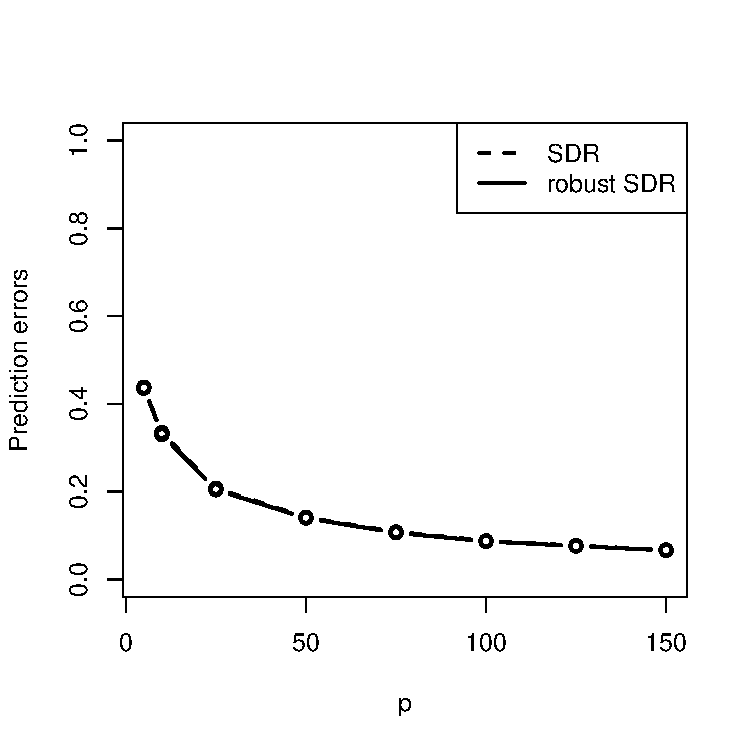
\includegraphics[width=0.35\textwidth]{SDRcomparison_noout}
	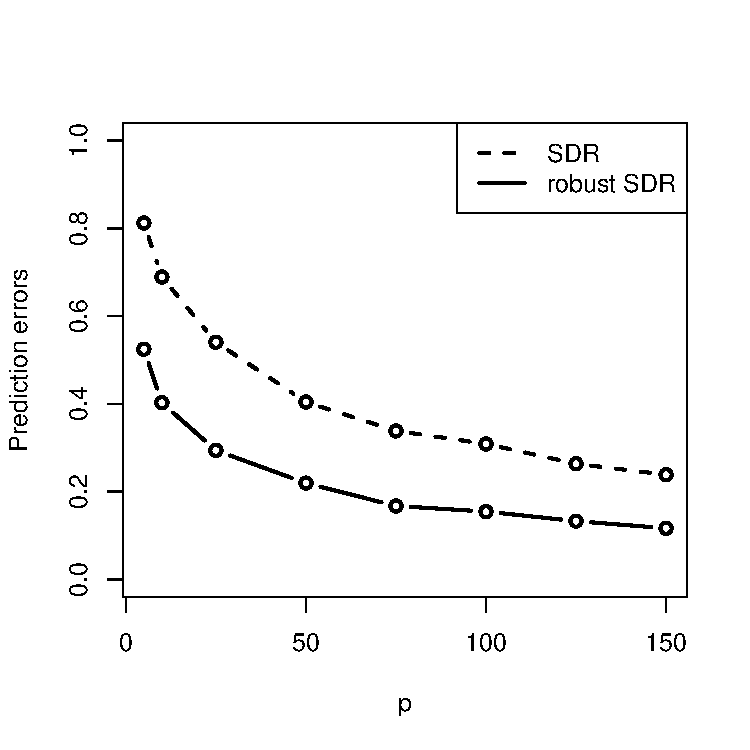
\includegraphics[width=0.35\textwidth]{SDRcomparison_out}
	\caption{Plot of the norm of influence function for first eigenvector of (a) sample covariance matrix, (b) SCM, (c) Tyler's scatter matrix and DCMs for (d) Halfspace depth, (e) Mahalanobis depth, (f) Projection depth for a bivariate normal distribution with $\bfmu = {\bf 0}, \Sigma = \diag(2,1)$}
	\label{fig:SDRfig}
\end{figure}

We formulate a robust version of the above procedure by estimating the quantities $\bfGamma, \bar\bfmu, \bfmu_y, \sigma^2$ by robust methods. Specifically, we take the following as their estimates:
%
\begin{itemize}
\item $\hat {\tilde \bfGamma}_d = $ first $d$ eigenvectors of the sample DCM;
%
\item $\hat \bfmu_s = $ spatial median of the rows of the data matrix $\BX_n$;
%
\item $\hat \bfmu_{s,y} = $ spatial median of the rows of $ \BX_y = \BX_n | Y=y$, for all $y \in S_Y$;
%
\item $\tilde\sigma^2 = \sum_{j=1}^p [\widehat{\text{MAD}}_Y (\BX_{Y,j} - \hat \mu_{s,j} - \hat {\tilde \bfgamma}_{d,j}^T \tilde \bfv_Y)]^2/p$, with $\hat {\tilde \bfGamma}_d = (\hat {\tilde \bfgamma}_{d,1}, ..., \hat {\tilde\bfgamma}_{d,p} )^T$, and MAD being the median absolute deviation.
\end{itemize}
%
The following simulation study using the same setup as in \citep{AdragniCook09} compares the performance of our robust SDR with the original method with or without the presence of bad leverage points in the covariate matrix $\BX_n$. For a fixed dimension $p$, we take $n=200, d=1$, generate the responses $Y$ as independent standard normal, and the predictors as $\BX_Y = \bfgamma^* v_Y^* + \bfepsilon$, with $\bfgamma^*_{p\times 1} = (1,...,1)^T, v_Y = Y + Y^2 + Y^3$ and $ \BV (\bfepsilon) = 25 \bfI_p$. We measure performance of both SDR models by their mean squared prediction error on another set of 200 observations generated similarly, and taking the average of these errors on 100 such training-test pair of datasets. Finally we repeat the whole setup for different choices of $p = 5,10,25,50,75,100,125,150$.

Panel (a) of \ref{fig:SDRfig} compares prediction errors using robust and maximum likelihood SDR estimates when the covariate matrix contains no outliers, and the two methods are virtually indistinguishable. We now introduce outliers in each of the 100 datasets by adding 100 to first $p/5$ coordinates of the first 10 samples in $\BX_n$, and repeat the analysis. Panel (b) of the figure shows that although our robust method performs slightly worse than the case when there were no outliers, it remains more accurate in predicting out-of-sample observations for all values of $p$. 